\documentclass[aspectratio=169]{beamer}

\usepackage{beamerthemesplit}
\usepackage{amsmath}
\usepackage{amsfonts}
\usepackage{amssymb}
\usepackage{cancel}
\usepackage{bussproofs}
\usepackage{graphicx}

% For ⩘ and ⩗ (requires the LuaLaTeX engine)
\usepackage{unicode-math}
\setmathfont{Stix Two Math}

% For highlighting MeTTa code
\usepackage{listings}
\usepackage{color}
\definecolor{mygreen}{rgb}{0,0.6,0}
\definecolor{mygray}{rgb}{0.5,0.5,0.5}
\definecolor{mymauve}{rgb}{0.58,0,0.82}
\lstset{ %
  backgroundcolor=\color{white},   % choose the background color
  basicstyle=\tiny,                % size of fonts used for the code
  breaklines=true,                 % automatic line breaking only at whitespace
  captionpos=b,                    % sets the caption-position to bottom
  commentstyle=\color{mygreen},    % comment style
  escapeinside={\%*}{*)},          % if you want to add LaTeX within your code
  keywordstyle=\color{blue},       % keyword style
  stringstyle=\color{mymauve},     % string literal style
}

% Commands for Atomese code
\newcommand{\SP}{\;\;\;}
\newcommand{\TTrue}{\textit{True}}
\newcommand{\TFalse}{\textit{False}}
\newcommand{\TAtom}{\textit{Atom}}
\newcommand{\TTime}{\textit{Time}}
\newcommand{\TEval}{\textit{Evaluation}}
\newcommand{\TList}{\textit{List}}
\newcommand{\TLamb}{\textit{Lambda}}
\newcommand{\TExec}{\textit{Execution}}
\newcommand{\TAtTime}{\textit{AtTime}}
\newcommand{\TAnd}{\textit{And}}
\newcommand{\TOr}{\textit{Or}}
\newcommand{\TNot}{\textit{Not}}
\newcommand{\TImpl}{\textit{Implication}}
\newcommand{\TPredImpl}{\textit{PredictiveImplication}}
\newcommand{\TSeqAnd}{\textit{SequentialAnd}}
\newcommand{\TSeqOr}{\textit{SequentialOr}}
\newcommand{\TBSeqAnd}{\textit{BackSequentialAnd}}
\newcommand{\TFSeqAnd}{\textit{ForeSequentialAnd}}
\newcommand{\TLag}{\textit{Lag}}
\newcommand{\TLead}{\textit{Lead}}
\newcommand{\TTV}{\textit{TV}}
\newcommand{\TTVo}{\textit{TV}_1}
\newcommand{\TTVi}{\textit{TV}_i}
\newcommand{\TTVn}{\textit{TV}_n}
\newcommand{\TTVPo}{\textit{TV}_1^P}
\newcommand{\TTVQo}{\textit{TV}_1^Q}
\newcommand{\TTVPi}{\textit{TV}_i^P}
\newcommand{\TTVQi}{\textit{TV}_i^Q}
\newcommand{\TTVPn}{\textit{TV}_n^P}
\newcommand{\TTVQn}{\textit{TV}_n^Q}
\newcommand{\TTVP}{\textit{TV}^P}
\newcommand{\TTVQ}{\textit{TV}^Q}
\newcommand{\TTVR}{\textit{TV}^R}
\newcommand{\TTVPQ}{\textit{TV}^{PQ}}
\newcommand{\TTVQR}{\textit{TV}^{QR}}
\newcommand{\TBTV}{\langle \TTV \rangle}
\newcommand{\TBTVPo}{\langle \TTVPo \rangle}
\newcommand{\TBTVQo}{\langle \TTVQo \rangle}
\newcommand{\TBTVPi}{\langle \TTVPi \rangle}
\newcommand{\TBTVQn}{\langle \TTVQn \rangle}
\newcommand{\TBTVPn}{\langle \TTVPn \rangle}
\newcommand{\TBTVQi}{\langle \TTVQi \rangle}
\newcommand{\TBTVP}{\langle \TTVP \rangle}
\newcommand{\TBTVQ}{\langle \TTVQ \rangle}
\newcommand{\TBTVR}{\langle \TTVR \rangle}
\newcommand{\TBTVPQ}{\langle \TTVPQ \rangle}
\newcommand{\TBTVQR}{\langle \TTVQR \rangle}
\newcommand{\Tstrength}{\textit s}
\newcommand{\Tconf}{\textit c}

% Commands for symbolic mathematical notations
\newcommand{\prob}[1]{\mathcal{Pr}\left(#1\right)}
\newcommand{\mean}{\textit{mean}}
\newcommand{\cnt}{\textit{count}}
\newcommand{\poscnt}{\textit{pos\_count}}
\newcommand{\sat}[1]{\mathcal{S}(#1)}
\newcommand{\ltv}[1]{<\!\!#1\!\!>}
\newcommand{\letv}[2]{(#1, #2)}
\newcommand{\limp}{\rightarrow}
\newcommand{\lpreimp}[1]{\leadsto^{#1}}
\newcommand{\lseqor}[1]{\bigslopedvee^{#1}}
\newcommand{\lseqand}[1]{\bigslopedwedge^{#1}}
\newcommand{\lbseqor}[1]{\reflectbox{$\bigslopedvee$}^{#1}}
\newcommand{\lbseqand}[1]{\reflectbox{$\bigslopedwedge$}^{#1}}
\newcommand{\ldo}[1]{\widehat{#1}}
\newcommand{\llag}[2]{\overrightarrow{#1}^{#2}}
\newcommand{\llead}[2]{\overleftarrow{#1}^{#2}}

\makeatletter
\newcommand*{\dashdownarrow}{%
  \mathrel{%
    \mathpalette\dasharrow@vert{-90}%
  }%
}
\newcommand*{\dashuparrow}{%
  \mathrel{%
    \mathpalette\dasharrow@vert{90}%
  }%
}
\newcommand*{\dasharrow@vert}[2]{%
  \sbox0{$#1\vcenter{}$}%
  \sbox2{$#1\dashrightarrow\m@th$}%
  \dimen@=1.2\dimexpr\ht2-\ht0\relax
  % 1/2 width of the new symbol with side bearing
  \sbox2{\raisebox{-\ht0}{\unhcopy2}}%
  \ht2=\z@
  \dp2=\z@
  \vcenter{\hbox to 2\dimen@{\hfill\rotatebox{#2}{\box2}\hfill}}%
}
\makeatother

\makeatletter
\newcommand{\reallytiny}{\@setfontsize{\srcsize}{2pt}{2pt}}
\makeatother

\mode<presentation>
{
  \usetheme{AnnArbor}
  \usecolortheme{crane}
}

\usepackage[english]{babel}
%% \usepackage[latin1]{inputenc}
\usepackage{times}
\usepackage[T1]{fontenc}

\title{Probabilistic Logic Networks for Temporal and Procedural Reasoning}

\author{Nil Geisweiller, Hedra Yusuf}

\institute[SingularityNET OpenCog Foundations]
{
  \begin{center}
    Artificial General Intelligence 2023 (AGI-23)\\
    
\includegraphics[scale=0.32]{pictures/snet_oc.png}
  \end{center}
}

\date[AGI-23]

\begin{document}

\section{Introduction}

\begin{frame}
  \maketitle

  % <BEGIN-SPEECH>
  % I'm going to present an extension of PLN (Probabilistic Logic
  % Networks) for temporal and procedural reasoning.  It is based on
  % the PLN book but with some differences and it comes with a proper
  % formalization.
  % <END-SPEECH>
\end{frame}

\section{PLN Recall}

\begin{frame}
  % <BEGIN-SPEECH>
  % Let me begin with a short and partial recall of PLN.  PLN is a
  % logic that has been created by Ben Goertzel, Matt Ikle and a few
  % others, to ultimately capture the kind of common sense reasoning
  % that humans uses in order to navigate the world and deal with its
  % uncertainty.  It's very similar to NAL (Non-Axiomatic Logic from
  % Pei Wang) but it is based on probability theory.
  % <END-SPEECH>

  % <BEGIN-SPEECH>
  % We have predicates, so functions that go from a certain domain to
  % Boolean.  These are however probabilistic, first in the sense that
  % a second order probabilistic distribution can be attached to a
  % predicate to measure its prevalence of being true.  A second order
  % probabilistic distribution, is a probability over a probability
  % and is used to represent the uncertainty of probabilities.  An
  % easy way to represent a second order distribution is with a
  % Beta-distribution, which has interesting mathematical properties
  % as well, and in PLN such distribution is represented by two
  % numbers, a strength, here s, and a confidence, here c.  Predicates
  % are also probabilistic in the sense that each individual
  % evaluations of that predicate can have a second order probability
  % attached to it as well.  We have relationships over predicates,
  % such as implication, corresponding to a form of second order
  % conditional probability.  We have the usual connectors, and, or,
  % not, corresponding to intersection, union and complement.
  % <END-SPEECH>

  \begin{columns}
    \column{7.8cm}

    \underline{Predicates and Connectors}:
    \begin{itemize}
    \item<+-> $P, Q, R, \hdots: \textit{Domain} \mapsto \{\TTrue, \TFalse\}$
    \item<+-> $P(a) \measeq\ <\!s\ c\!>$
    \item<+-> $P \measeq\ <\!s\ c\!> \ \ \ \ \ \ \ \ \ \ \ \ \ \equiv \ \ \ \ \prob{P} \approx s$
    \item<+-> $P \rightarrow Q \measeq\ <\!s\ c\!> \ \ \ \ \ \equiv \ \ \
      \ \prob{P|Q} \approx s$
    \item<+-> $P \land Q \measeq\ <\!s\ c\!> \ \ \ \ \ \ \ \! \equiv \ \ \ \prob{P
        \cap Q} \approx s$
    % \item<+-> $P \lor Q \measeq\ <\!s\ c\!> \ \ \ \ \ \ \ \! \equiv \ \ \ \prob{P
    %     \cup Q} \approx s$
    \item<+-> $\lnot P \measeq\ <\!s\ c\!> \ \ \ \ \ \ \ \ \ \ \! \ \equiv \ \ \
      \prob{\overline{P}} \approx s$
    \end{itemize}

    \column{7cm}

    \visible<2->{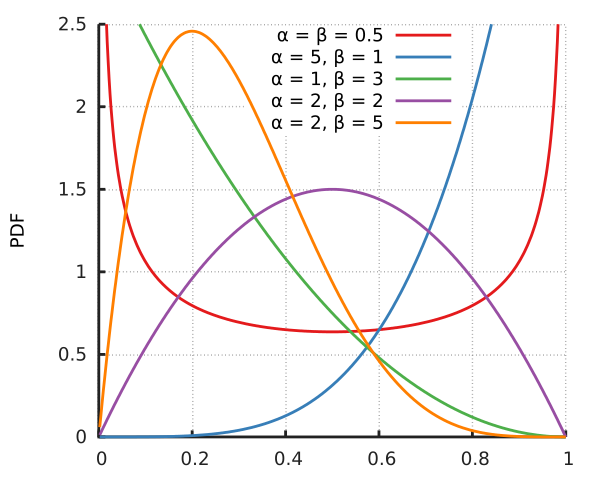
\includegraphics[scale=0.25]{pictures/600px-Beta_distribution_pdf.svg.png}}

  \end{columns}

  \pause
  \underline{Inference Rules}:
  \pause

  \begin{itemize}
  \item<+-> Implication Direct Introduction (IDI)
    {\small
      \begin{prooftree}
        \AxiomC{$P(a_1) \measeq \TTVPo$}
        \AxiomC{$Q(a_1) \measeq \TTVQo$}
        \AxiomC{$\hdots$}
        \AxiomC{$P(a_n) \measeq \TTVPn$}
        \AxiomC{$Q(a_n) \measeq \TTVQn$}
        \RightLabel{(IDI)}
        \QuinaryInfC{$P\limp Q \measeq \phi_{IDI}\left(\TTVPo, \dots, \TTVQn\right)$}
      \end{prooftree}}

  \item<+-> Deduction (D)
    {\small
      \begin{prooftree}
        \AxiomC{$P \limp Q \measeq \TTVPQ$}
        \AxiomC{$Q \limp R \measeq \TTVQR$}
        \AxiomC{$P \measeq \TTVP$}
        \AxiomC{$Q \measeq \TTVQ$}
        \AxiomC{$R \measeq \TTVR$}
        \RightLabel{(D)}
        \QuinaryInfC{$P \limp R \measeq \phi_D\left(\TTVPQ, \dots, \TTVR\right)$}
      \end{prooftree}
    }
  \end{itemize}

\end{frame}

\section{Temporal PLN}

\section{Procedural PLN}

\end{document}
